\documentclass[journal]{IAENGtran}

\ifCLASSINFOpdf
   \usepackage[pdftex]{graphicx}
   \DeclareGraphicsExtensions{.pdf,.jpeg,.png}
\else
   \usepackage[dvips]{graphicx}
   \DeclareGraphicsExtensions{.eps}
\fi

\begin{document}
\title{An Explanation Method of Unfamiliar Tourist Spots based on Roles of User's Familiar Spots}
\author{Kenta~Han, Daisuke~Kitayama

\thanks{Manuscript received December 20, 2018; revised January 10, 2019. }
\thanks{This work was supported by ISPS KAKENHI of Grant-in-Aid for Scientific Research(C) Grant Number 18K11551. }
\thanks{K. T. Han is with the Graduate School of Engineering, Kogakuin University, Japan; e-mail: em18011@ns.kogakuin.ac.jp.}% <-this % stops a space
\thanks{D. Kitayama is with the Faculty of Informatics, Kogakuin University, Japan;  e-mail: kitayama@cc.kogakuin.ac.jp.}}% <-this % stops a space


\maketitle

\pagestyle{empty}
\thispagestyle{empty}

\begin{abstract}
% 多くの観光客は,レジャー旅行を計画するときに,オンラインから利用可能情報を得ている.しかし,旅行客は未訪問エリアに向けられるかもしれないので,この頼りはしばしば問題を生じそして誤解を招くようになる.
Most tourists resort to available information online when planning for leisure travel; however, this recourse often becomes problematic and misleading as tourist of the information may be directed to unfamiliar areas.
% この点に関して,我々は彼らが既に訪れたことがあるスポットの特徴を通して未訪問スポットを説明する方法を提案した.
On this regard, we proposed a method of explaining unfamiliar spots through the familiar features of spots they have visited.
% 本研究では,まず,観光スポットのユーザレビューを用いて特徴ベクトルを生成した.
In this paper, at first, we generated the feature vector using user reviews of the tourist spot.
% 次に,既に訪問したスポットと比較した相対的な特徴ベクトルを用いて,観光スポットの独特な特徴を抽出した.
Next, we used the relative feature vector compared with already visited spots to extract the role of the tourist spot for the user.
% 最後に,相対的特徴ベクトルの類似性によって訪問スポットを未訪問スポットと関連付け,さらにその関係を説明するキーワードを抽出した.
Finally, we associated the visited spot with the unfamiliar spot by the similarity of the relative feature vector, and further extracted keywords that explain the relation.
% また,システムのプロトタイプを開発し,既訪問スポットと未訪問スポットの間の説明情報の効果を評価した.
Furthermore, we developed a prototype of the system and evaluated the effect of the explanatory information between the familiar and unfamiliar spots.
\end{abstract}

\begin{IAENGkeywords}
Tourist spots, explainability, tourist reviews, paragraph vector
\end{IAENGkeywords}

\IAENGpeerreviewmaketitle

%%%%%%%%%%%%%%%%%%%%%%%%%%%%%%%%%%%%%%%%%%
%%%%%%%%%%%%%%%%%%%%%%%%%%%%%%%%%%%%%%%%%%
\section{Introduction}
\label{sec:Introduction}
% 旅行先を決定する時,旅行者はWeb情報を頼る場合が多くなっている.
\IAENGPARstart{T}{ourists} often resort to web information when planning travel destinations.
% 出版されたガイドの正確さはしばしば信頼できず,旅行者が未訪問エリアで迷子になる可能性が高くなる.
The accuracy of these published guides is oftentimes unreliable and leads to the high probability of the traveler getting lost in an unfamiliar area.
% 現時点では,ほとんどの観光客が彼らが訪問を検討しているスポットに関するオンラインレビュー,旅行やレジャーのコミュニティのランキング,そして検索エンジンの推奨を読んでいる.
At present, most tourists read online reviews, travel and leisure communities ranking, and search engine recommendations regarding the spots they consider visiting.
% % 例えば,人気のある日本の観光スポット投稿サイトTripadvisorとJalanは行き先のレビューや旅行者からの経験に関する豊富な情報を提供している.
% For instance, popular Japanese tourist spot posting sites Tripadvisor\footnote{https://www.tripadvisor.com/} and Jalan\footnote{Jalan https://www.jalan.net/kankou/} offer a wealth of information on destination reviews and experiences from travelers.
% Tripadvisorやじゃらんなどの観光スポット検索サイトでは,ユーザが特定の観光スポットを訪問した後レビューを投稿するため,観光スポットに関する豊富な情報がある.
In a tourist spot search engine such as Tripadvisor\footnote{https://www.tripadvisor.com/} and Jalan\footnote{Jalan is a review posting site on tourist spots in Japan. https://www.jalan.net/kankou/}, the tourist who visited there about a certain tourist spot posted reviews and there is a wealth of information on tourist spots.
% しかし,ユーザは訪問したいエリアについての事前知識がないため,検索された観光スポットを1つずつ確認する必要がある.
However, since the tourist has no prior knowledge about the search area, what kind of tourist spot is to be confirmed one by one.
% さまざまな観光スポットを効果的に理解するためには,既存の情報をもとにして,未知な情報と既知な情報との対応関係を考えることが不可欠となる.
Therefore, in order to effectively understand various tourist spots, we think that it is effective if we compare an unfamiliar spot using a visited spot of tourist.
% 代替案として,我々は,ユーザが既訪問スポットを使用し,未訪問スポットに対する効果的なロケータ技法を提案した.
As an alternative, we proposed an effective locator technique for an unfamiliar spot using a spot visited and familiar to the user.
% % このアプローチは,現在の問題に対する経験の採用に似ている.
This approach is analogous to employing experience over the current problem.
% さらに解明するために,以前の経験は既訪問スポット,現在の問題は未訪問スポットである.
To elucidate further, the previous experience indicates the familiar spot and the current problem is the unfamiliar spot.
% 例えば,日本の東京の「表参道」のような未訪問スポットは,パリでは「アベニューデシャンゼリゼ通り」と表現されていると,フランス人の初心者にとっては見つけやすく理解しやすいかもしれません,彼らが訪問し,後者の分野に精通しているとする.
For instance, unfamiliar spots such as ``Omotesando'' in Tokyo, Japan may be located and understood easier by a newcomer French user when it is described as ``Avenue des Champs-Elysees'' in Paris, given that he/she has visited and is familiar with the latter area.

% 提案手法では,ユーザは既に訪れたことがある場所や未訪問エリアを入力する.
In the proposed method, the user inputs already visited and unfamiliar area.
% これから,観光スポットのユーザレビューに基づいて特徴ベクトルが生成する.
From this, a feature vector is generated based on user reviews of the tourist spot.
% 次に,ユーザの観光地の役割を抽出するために,既に訪れたスポットと比較した相対的特徴ベクトルを使用する.
Next, we use the relative feature vector compared with already visited spots to extract the role of the tourist spot for the user.
% 最後に,訪問されたスポットは,それらの相対的特徴ベクトルの類似性によって未訪問スポットと関連付けられ,そして関係を説明するキーワードが抽出される.
Finally, the visited spot is associated with the unfamiliar spot by similarity of their relative feature vector, and keywords that explain the relation are further extracted.
% このようにして,未訪問スポットに対するユーザーの理解を深める.
This way, we aim to enhance user understanding of unfamiliar spots.
% 提案された方法の概念を図\ref{fig:Photo_Image}に示す.
Figure \ref{fig:Photo_Image} shows the concept of the proposed method.

% この論文の残りの部分は次のように構成されている.
The rest of the paper is structured as follows.
% \ref{sec:Related Work}節ではコンセプトに関する関連研究を紹介し,\ref{sec:An Explanation Method of Unfamiliar Tourist Spots}ではその方法を説明している.
Section \ref{sec:Related Work}, introduces related works on the concept, while Section \ref{sec:An Explanation Method of Unfamiliar Tourist Spots} describes the method.
% 評価実験とその結果は\ref{sec:Evaluation Experiment}節で議論されている.
Evaluation experiments and their results are discussed in Section \ref{sec:Evaluation Experiment}.
% 最後に,\ref{secsec:Conclusions and Future Work}では,この論文の結論と今後の課題について説明する.
Finally, Section \ref{sec:Conclusions and Future Work}, presents the conclusions of the paper and our future work.

%%%%%%%%%%%%%%%%%%%%%%%%%%%%%%%%%%%%%%%%%%
%%%%%%%%%%%%%%%%%%%%%%%%%%%%%%%%%%%%%%%%%%
\section{Related Work}
\label{sec:Related Work}
%%%%%%%%%%%%%%%%%%%%%%%%%%%%%%%%%%%%%%%%%%
\subsection{Tourist spot retrieval and recommendation system}
\label{subsec:Tourist spot retrieval and recommendation system}
% 利用者の経験履歴を用いた検索推薦システムに関する研究がいくつか発表されている.
Several research on retrieval and recommendation system using user's experience history have been published.
% 倉島ら\cite{Codd01}は,Flickrに投稿された集約写真のジオタグ情報を用いた旅行ルートの推薦方法を提案した.この手法では,時間情報で分類すると個人的な旅行履歴と見なすことができる.
Kurashima et al.\cite{Codd01} proposed a travel route recommendation method using geotag information of aggregated photos posted at Flickr, which could be regarded as personal travel history when sorted by time information.
% この方法では,利用者の現在地から自分の興味を引きやすい場所へ移動することを想定し,ジオタグ情報を用いて行動モデルを生成した.
In this method, moving from a user's present location to a place easily accessible to his/her interest was presumed, and a behavior model was generated using the geotag information.
% 北村ら\cite{Codd02}は,一般的な物体認識システムを使用して過去の個人旅行写真から旅行プランのユーザの好みを推定し、写真から撮影した被写体情報のキーワードを取得することによって観光スポットを推薦した.
Kitamura et al.\cite{Codd02} recommended sightseeing spots by estimating user's preferences of travel plan from past personal travel photographs using a general object recognition system to acquire keywords of subject information taken from the photos.
% また,彼女らは旅行写真でグラフを視覚化するユーザインタフェースを提示するグラフ視覚化技術によってキーワードの共起を表現した.
Moreover, she represented the co-occurrence of the keywords by a graph visualization technique, which presents a user interface that visualizes a graph with travel photos.
% 反対に,Chengら\cite{Codd03}は,提案された特定のユーザプロファイルや属性を考慮して,自由に利用可能なコミュニティ投稿の写真を使ってパーソナライズされた旅行の推奨に焦点を当てた.
Conversely, Cheng et al.\cite{Codd03} used photographs of freely available community contributions to focus on personalized trip recommendations, considering suggested specific user profiles or attributes.

%%%%%%%%%%%%%%%%%%%%%%%%%%%%%%%%%%%%%%%%%%
\subsection{The analogy and its applications}
\label{subsec:The analogy and its applications}
% 類推は創造的思考に貢献すると指摘されてた\cite{Codd04},既知の知識(ベースと呼ぶ)から概念(ターゲットと呼ぶ)を獲得するときに類推思考が働くとされる\cite{Codd05}.
Analogies were pointed out as contributing to creative thinking\cite{Codd04}; analogical thinking works when acquiring a concept (called the target) from known knowledge (called the bases)\cite{Codd05}.
% 類推に関する研究の多くは,ベースとなる学習データとターゲットとなる問題が与えられ,物事の特徴を問題の特徴にマッピングして問題を解決するもの\cite{Codd06}である.
Many research on analogy were given the base learning data and targeted problems, and the problems were solved by mapping the features of things to the feature of the problem\cite{Codd06}.
% Gickらは,不確定な問題の解を見つけるためのガイドとして,異種ドメイン間の類推の使用を調査するように設計した.
Gick et al. investigated the use of analogies between disparate domains as a guide to finding solutions for an ill-defined problem.
% 学習データの与え方や機能について研究したもの\cite{Codd07}や,認知的な熟達度に応じて問題を解決するかどうかを明らかにしたもの\cite{Codd08}がある.
Some studied on how to give learning data and functions\cite{Codd07}, and clarified whether to solve the problem depending on the degree of cognitive proficiency\cite{Codd08}.
% これらを含む従来研究の多くにおいては,類推に用いるベースとターゲットを与えたあとで,問題にある手順に従って解決された.
In many of the conventional research including these, after giving bases and targets for analogy, problems were solved according to a certain procedure.
% 構造の類似性には3種類あり,特徴の共有数で決まる「対象レベルの類似性」,ベースに存在する関係とターゲットに存在する関係の共有度に基づく「関係レベルの類似性」,および題の解法あるいは目標レベルでの類似性である「プラグマティックな類似性」とがある\cite{Codd05},\cite{Codd09}.
There are three types of structural similarities: ``similarity of object level'' determined by the number of shared features, ``relationship similarity'' based on the degree of sharedness of relationships existing in the base and the relationship existing in the base, and ``pragmatic similarity'' based on the title solution or target level \cite{Codd05},\cite{Codd09}.

% ユーザの経験履歴を使用する従来の方法では,いくつかの研究が履歴写真のジオタグ情報を分析し,それらをユーザの好みに変換した.類推技術も学習と理解を支援するために利用された.
In the conventional method of using the user's experience history, several research analyzed the geotag information of the history photograph and converted them into user's preference; analogy techniques were also utilized to support learning and understanding.
% 本研究では,地域情報の理解を深めるために,既訪問スポットと未訪問スポットの見直し,および各スポットの相対的な特徴を見分け,関連付けを行った.
In this research, a review of familiar spots and unfamiliar spots and the relative features of each spot, via the sets of spots familiar and unfamiliar to the user, were determined and associated to enhance understanding of the area information.
% それが明示的に類推を利用したので,この論文は「関係レベルの類似性」と同様の構造を持つと推定される.
As it exploited analogy explicitly, this paper is presumed to have similar structure as with the ``similarity of relationship level."

\begin{figure}[t]
  \begin{center}
    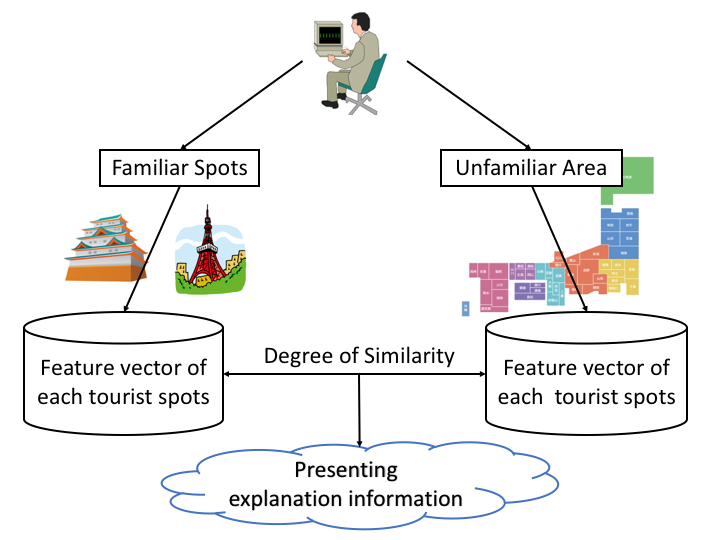
\includegraphics[clip,width=7.5cm,bb=0 0 720 540]{picture/Photo_Image_eng.png}
    \caption{An explanation method of unfamiliar tourist spots based on roles of user's familiar spots}
    \label{fig:Photo_Image}
   \end{center}
\end{figure}

%%%%%%%%%%%%%%%%%%%%%%%%%%%%%%%%%%%%%%%%%%
%%%%%%%%%%%%%%%%%%%%%%%%%%%%%%%%%%%%%%%%%%
\section{An Explanation Method of Unfamiliar Tourist Spots}
\label{sec:An Explanation Method of Unfamiliar Tourist Spots}
% In this method, the user inputs a set of tourist spots he/she has visited and the destination he/she intends to visit. Next, a feature vector is generated based on user reviews of the intended tourist spot. Afterwards, a feature vector relative to the visited spots is used for extraction of their role to the intended destination of the user. The relative feature vector of each tourist spot in the unfamiliar area is calculated and compared. Finally, the relative feature vector of the unfamiliar spot is associated to the similar feature vector of the visited spot, and the keywords explaining the relation are extracted.
% 我々は,ユーザの既訪問スポットの位置づけに基づく未訪問スポットの説明手法を提案する.
We propose an explanation method of unfamiliar tourist spots based on roles of user's familiar spots.
% まず,ユーザが既訪問の複数個の観光スポットと訪問したい観光スポットエリア情報を入力する.
At first, the user inputs a set of tourist spots that have been visited and tourist area that user wishes to visit.
% 本手法では,観光スポットのユーザレビューを用いて特徴ベクトルを作成する.
In our method, we generate the feature vector using user reviews of the tourist spot.
% 次に,ユーザの観光地の役割を抽出するために,既に訪れたスポットと比較した相対的特徴ベクトルを使用する.
Next, we use the relative feature vector compared with already visited spots to extract the role of the tourist spot for the user.
% 同様に,未訪問エリアの各観光スポットの相対的な特徴ベクトルを,そのエリアの他の観光スポットと比較して計算する.
Similarly, we calculate the relative feature vector of each tourist spot in the unfamiliar area by comparing with other tourist spots in that area.
% 次に,相対的な特徴ベクトルの類似性によって訪問されたスポットを未訪問スポットと関連付ける.
Then, we associate the visited spot with the unfamiliar spot by the similarity of the relative feature vector.
% 最後に,その関係性を説明するためのキーワードを抽出する.
Finally, we extract keywords that explain the relation.

%%%%%%%%%%%%%%%%%%%%%%%%%%%%%%%%%%%%%%%%%%
\subsection{Generating feature vector using user reviews of spot}
\label{subsec:Generating feature vector using user reviews of spot}
% 2016年9月末まで,「Jalan」から取得したレビューデータを使用した.
We used the review data obtained from ``Jalan'' until the end of September 2016.
% 分散表現\cite{Codd10}を使って観光地の特徴ベクトルを生成しした.我々は観光地のすべてのレビューをまとめ,それらを1つの文書として扱った.
We generated feature vectors of tourist spots using paragraph vector\cite{Codd10}; we combined all reviews on a tourist spot and treated them as one document.
% 分散表現を計算するにはgensimというPythonライブラリを使用し,学習方法としては300次元の分散Bag-of-Wordsを使用した.
We used a Python library called gensim\footnote{https://radimrehurek.com/gensim/models/doc2vec.html} to calculate the paragraph vector, and the Distributed Bag-of-Words with 300 dimensions as the learning method.
% Jalanでのユーザレビューは日本語で書かれているので,MeCab \cite{Codd11}を辞書の `` mecab-ipadic-NEologd ''を付けて日本語の形態素解析ツールとして使用した.
As user reviews in Jalan are written in Japanese, we used MeCab\cite{Codd11} as the Japanese morphological analyzer with dictionary ``mecab-ipadic-NEologd''\footnote{https://github.com/neologd/mecab-ipadic-neologd/}.

%%%%%%%%%%%%%%%%%%%%%%%%%%%%%%%%%%%%%%%%%%
\subsection{Relative features for role of tourist spots}
\label{Relative features for role of tourist spots}

\begin{figure}[t]
  \begin{center}
    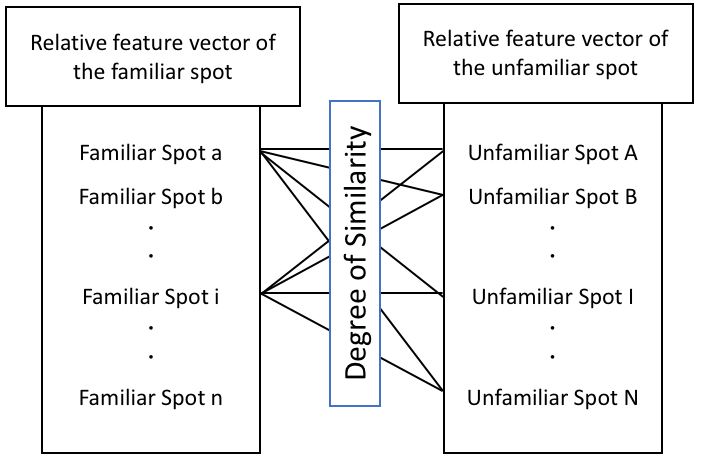
\includegraphics[clip,width=7.5cm,bb=0 0 702 458]{picture/Photo_CosSim_eng.png}
    \caption{Concept of similarity calculation}
    \label{fig:Photo_CosSim}
  \end{center}
\end{figure}

% 我々は,他の観光地間の相対的な特徴を比較することによって観光地の役割を抽出した.
We extracted the role of tourist spots by comparing their relative features with those of other tourist spots.
% 相対的特徴は,観光スポット集合の平均的特徴と比較される目標スポットの特徴として定義される.
A relative feature is defined here as the feature of the target spot that is compared to the average feature of a set of tourist spots.
% たとえば,日本の有名な観光スポット集合にある「東京都庁舎展望台」と「金閣寺」を検討する.
For example, we could consider ``the Tokyo Metropolitan Government Building Observatories (TMGBO)'' and ``Kinkakuji Temple'' under a set of famous tourist spots in Japan.
% 「金閣寺」の相対的な特徴は,寺院,金色,京都市などである.一方,「TMGBO」は,パノラマビュー,夜景,建物そのもの,新宿区などの特徴を持っているなどである.
The relative features of ``Kinkakuji Temple'' are the temple, its golden color, the city of Kyoto, and so on, while ``TMGBO'' has the features of panoramic view, night view, the building itself, the Shinjuku ward, and so on.
% 他の観光スポットと比較すると,2つの例の相対的な特徴は一般的な特徴,カテゴリ,および場所になる傾向がある.
When compared with other tourist spots, the relative features of the two examples tend to be general features, categories, and places.

% 他の例を見てみる.
Let us take another example.
% 日本の京都にある寺院の中にある「金閣寺」と「清水寺」を考える.
We could consider ``Kinkakuji Temple'' and ``Kiyomizudera Temple'' under a set of temples in Kyoto, Japan.
% 「金閣寺」の相対的な特徴は金色,金箔,輝きなどですが,「清水寺」では舞台やパノラマの景色などが特徴である.
The relative features of ``Kinkakuji Temple'' are its golden color, gold leaf, brilliance, and so on, while for ``Kiyomizudera Temple'' these features include the stage, the panoramic view, and so on.
% 両方の寺院は京都にあるので,京都と寺院に関連する特徴は相対的な特徴として現れません.代わりに,より詳細な機能が得られる.
As both temples are located in Kyoto, features related to Kyoto and temples do not appear as relative features; instead, more detailed features are obtained.

% 相対的特徴ベクトル$r_{state,i}$は,次のように自身の特徴ベクトルから他のスポットの特徴ベクトルの平均を減算することによって得らる.
The relative feature vector $r_{state,i}$ is obtained by subtracting the average of feature vectors of other spots from its own feature vector as in
\begin{equation}
  r_{state,i}=s_i-average(S_{state}-s_i),
  \label{math:Vector difference}
\end{equation}
% ここで,$S_{state} =\{s_1,s_2,\dots,s_n\}$は,$state$が$'f'$のときに設定されると未訪問スポットとなる.そうでなければ,$state$が$'u'$のときには未訪問スポットに設定される。
where $S_{state} =\{s_1,s_2,\dots,s_n\}$ is a familiar spot set when $state$ is $'f'$; otherwise, it is an unfamiliar spot set when $state$ is $'u'$.
% $s_i$という用語は,集合$S_{state}$内の観光地の特徴ベクトルである.
The term $s_i$ is a feature vector of a tourist spot in the set $S_{state}$.

\subsection{Determination of an explainable spot}
\label{subsec:Determination of an explainable spot}
% 未訪問エリア内のスポットは既訪問スポットを使って説明する.
We used a familiar spot to explain the spot in the unfamiliar area.
% 未訪問スポットと既訪問スポットを,既訪問スポット$r_{f,i}$と未訪問スポット$r_{u,j}$の相対的な特徴ベクトルによって計算される類似度を通して関連付けた(図\ref{fig:Photo_CosSim})
We associated unfamiliar spots and familiar spots through the similarity calculated by the relative feature vector of the familiar spot $r_{f,i}$ and the unfamiliar spot $r_{u,j}$ (Fig. \ref{fig:Photo_CosSim}).
% 類似度計算には,コサイン尺度を用いる.
We used the cosine scale below for the calculation
\begin{eqnarray}
  cos(r_{f,i},r_{u,j})=\frac{r_{f,i} \cdot r_{u,j}}{|r_{f,i}| \times |r_{u,j}|}.
  \label{math:CosSim}
\end{eqnarray}

% 関連付け手順は以下のように説明する,
The association procedure is explained as follows.
% まず,特定のスポットと最も類似度の高いスポットを関連付けた.
First, we associated a spot with the highest degree of similarity to a certain spot.
% 類似度が閾値(本論文では0.125)を下回ると,関連付けは行われない.
If similarity falls below the threshold (0.125 in this paper) then no association is made.
% 結果は,未訪問スポットと最も高い類似度を持つ既訪問スポットが関連付けられているか,既訪問スポットと最大の類似性を持つ未訪問スポットが関連付けられているかによって異なる.
The result depends on whether the familiar spot having the highest degree of similarity to the unfamiliar spot is associated, or the unfamiliar spot having the maximum similarity to the familiar spot is associated.
% 前者の条件では,すべての類似度が閾値を超えると,すべての既訪問スポットに対応するスポットがあるが,すべての未訪問スポットに対応するスポットがあるわけではない.
In the former condition, when all similarities exceed the threshold, all familiar spots have corresponding spots but not all unfamiliar spots have corresponding spots.
% 逆に,後者の場合,すべての類似性が閾値を超えたとき,すべての未訪問スポットに対応するスポットがある.
Conversely, in the latter case, when all similarities have exceeded the threshold, all unfamiliar spots have corresponding spots.
% 未訪問スポットについての説明を提供するために,我々は後者の条件を採用した.
To provide explanation for an unfamiliar spot, we adopted the latter condition.

%%%%%%%%%%%%%%%%%%%%%%%%%%%%%%%%%%%%%%%%%%
\subsection{Extraction of explainable words for role}
\label{subsec:Extraction of explainable words for role}
% 未訪問スポットと既訪問スポットとの間の関連性の観点を表すキーワードがユーザに提示された.
Keywords representing the viewpoints of association between the unfamiliar and familiar spots were presented to the user.
% しかし,相対的特徴ベクトルから単語の特徴を抽出することは不可能のため,我々は別の方法に頼った.
However, as extracting the feature of a word from the relative feature vector was not possible, we resorted to another method.
% 前提として,すべてのレビューは日本語の形態素解析ツールMeCabによって単語に分割された.ここでは,辞書として "mecab-ipadic-NEologd"を使用した.ただし,助詞,助動詞,副詞,記号,およびストップワードは削除された.
As a premise, all reviews were divided into words by the Japanese morphological analyzer MeCab, where we used ``mecab-ipadic-NEologd'' as the dictionary; however, the words particle, auxiliary verb, adnominal, symbol, and stop, were deleted.
% キーワード抽出では,まず対象となる既訪問スポットと未訪問スポットからTFIDF法により特徴語とTFIDF値を求めた.
For the keyword extraction, we first obtained a feature word and TFIDF value from the target familiar spot and unfamiliar spots by the TFIDF method.
% 次に,TFIDF値の調和平均を計算して,2つのスポットに共通の特徴語にスコアを付ける.
Next, we calculated the harmonic mean of the TFIDF values to score feature words common to the two spots.
% 最後に,説明文としてスコアの高い特徴語を抽出した.
Finally, we extracted the feature words with high scores as explainable words.

% スポット内のキーワードの特徴量は次の式で計算した.
We calculated the feature value of a keyword in a spot by the formula
\begin{equation}
  TFIDF(t,d,state) = TF(t,d) \times log\Biggr(\frac{|S_{state}|}{DF(t,state)}\Biggr),
  \label{math:TFIDF}
\end{equation}
% $TF(t,d)$は,文書$d$内のキーワード$t$の数を返す.これは,スポットのすべてのレビューを1つにまとめたものである.$DF(t,state)$は,キーワード$t$を含む文書の数を返す.$|S_{state}|$はスポットの総数である.
where function $TF(t,d)$ returns the number of the keyword $t$ in the document $d$, which combines all reviews of a spot into one; function $DF(t,state)$ returns the number of documents that include keyword $t$ and; $|S_{state}|$ is the total number of spots.
% $state$が$f$のときは,ユーザが入力した既訪問スポット集合を使用してTFIDF値を計算した.
When $state$ was $f$, we calculated TFIDF using a set of familiar spots from the user spot inputs.
% 同様に,$state$が$u$のときは,ユーザが入力したエリアに含まれている未訪問スポット集合を使用してTFIDF値を計算した.
Likewise when $state$ was $u$, we calculated TFIDF using the set of unfamiliar spots from the user area inputs.

% 2つのスポットに共通の特徴語のTFIDF値の調和平均を使用して,関連する既訪問スポットと未訪問スポットの説明可能なキーワードを抽出した.
We extracted the explainable keywords of the associated familiar and unfamiliar spots using the harmonic mean of the TFIDF values of the feature words common to the two spots.
% まず,既訪問スポットと未訪問スポットのレビュー文書によく現れる単語を抽出した.
First, we extracted words commonly appearing in the review document of the familiar and unfamiliar spots.
% 次にm抽出した単語のスコアを式\ref{math:Harmonic Mean}で計算した.$TFIDF(t,d,f)$と$TFIDF(t,d,u)$は,それぞれ既訪問スポットと未訪問スポットのTFIDF値を示している.
Next, we calculated the score of the extracted word by formula \ref{math:Harmonic Mean}. $TFIDF(t,d,f)$ and $TFIDF(t,d,u)$ indicate the TFIDF value of the familiar and unfamiliar spots, respectively.
% スコアが大きい場合,単語は各スポットで高い重要度を持ている.
The word has high importance in each spot when the score is large.
% したがって,スコアの上位N個の単語が説明情報としてユーザに提示された(Fig. \ref{fig:photo_map}),
Therefore, the top $N$ words of the score were presented as explanatory information to the user (Fig. \ref{fig:Photo_Map}).

\begin{eqnarray}
  score(t,d) = \frac{2 \times TFIDF(t,d,f) \times TFIDF(t,d,u)}{TFIDF(t,d,f) + TFIDF(t,d,u)}.
  \label{math:Harmonic Mean}
\end{eqnarray}

\begin{figure}[t]
  \begin{center}
    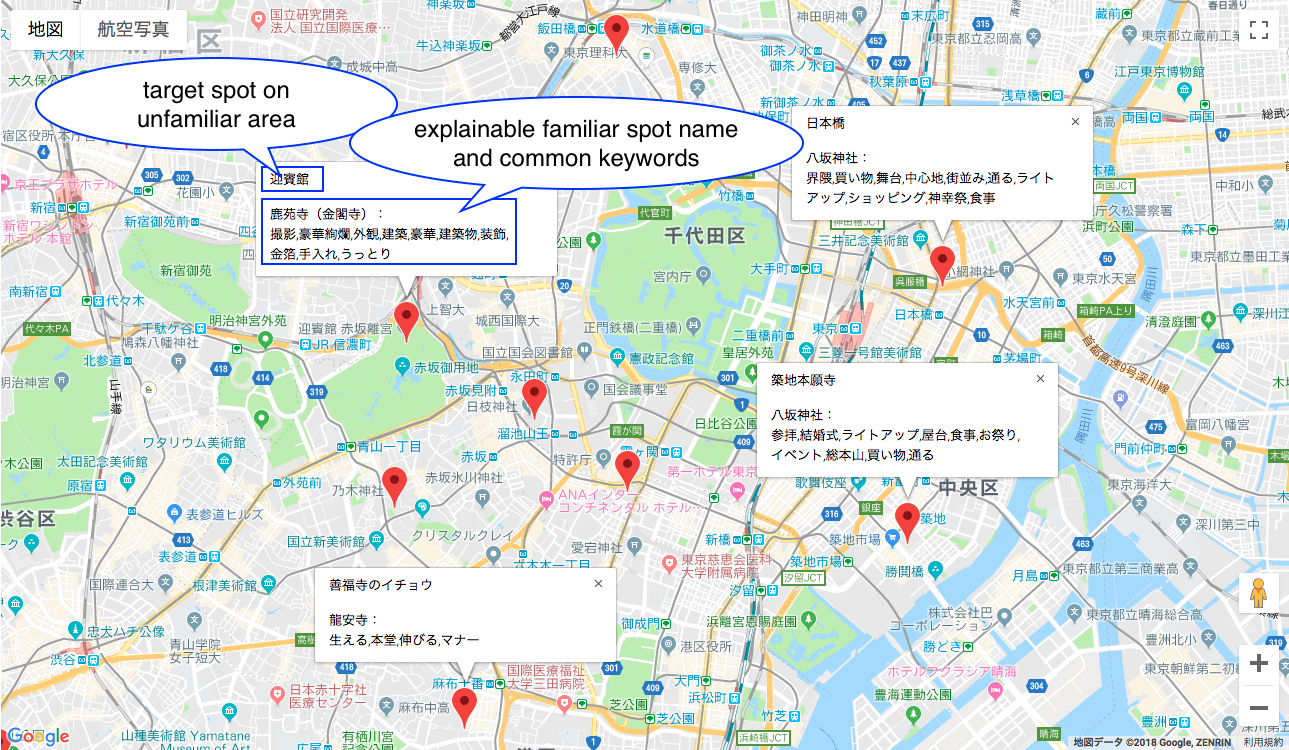
\includegraphics[clip,width=8.5cm,bb=0 0 1289 750]{picture/Photo_Map3_eng.png}
    \caption{User interface of prototype system}
    \label{fig:Photo_Map}
   \end{center}
\end{figure}

%%%%%%%%%%%%%%%%%%%%%%%%%%%%%%%%%%%%%%%%%%
\subsection{Example of explained unfamiliar spots}
\label{subsec:Example of explained unfamiliar spots}

\begin{table}[t]
  \caption{Set of Familiar and Unfamiliar spot}
  \label{table:Set of Familiar and Unfamiliar spot}
  \centering
  \begin{tabular}{l|l}
  \hline
  \multicolumn{1}{c|}{Familiar Spot Name} & \multicolumn{1}{c}{Unfamiliar Spot Name} \\ \hline
  Sensoji Temple                          & Tokyo Disneyland (R)                     \\
  Odawara-jo Park                         & Shinjuku Gyoen                           \\
  Fushimiinari-taisha Shrine              & Tokyo Skytree                            \\
  Nara Park                               & Tokyo Tower Main Deck            \\
  Mishima Skywalk                         & Meiji Jingu                              \\ \hline
  \end{tabular}
\end{table}

\begin{table*}[t]
  \caption{Explanation information}
  \label{table:Explanation information}
  \centering
  \begin{tabular}{l|l|l}
  \hline
  \multicolumn{1}{c|}{Unfamiliar Spot} & \multicolumn{1}{c|}{Familiar Spot} & \multicolumn{1}{c}{Explanation Information}                     \\ \hline
  Shinjuku Gyoen                      & Odawara-jo Park                         & flower viewing, bloom, inside the park, cherry-blossoms, leisurely, maintenance, nature, play equipment, azalea          \\
  Tokyo Skytree                     & Mishima Skywalk                    & Mt. Fuji, swing, high fear, ceiling, magnificent view, elevator, panorama, observation deck, rising
 \\ \hline
  \end{tabular}
\end{table*}

% 表\ref{table:Set of Familiar and Unfamiliar spot}は,ユーザの既訪問スポットと未訪問スポットの集合の例を示している.
Table \ref{table:Set of Familiar and Unfamiliar spot} shows an example of a set of user's familiar and unfamiliar spots.
% 東京では5つ未訪問スポットがランダムに選ばれた.
Five unfamiliar spots were randomly selected within Tokyo.
% 表\ref{table:Explanation information}は\ref{sec:An Explanation Method of Unfamiliar Tourist Spots}節で提案した方法を用いた説明可能な単語の一覧を示している.
Table \ref{table:Explanation information} shows the list of explainable words using the proposed method in Section \ref{sec:An Explanation Method of Unfamiliar Tourist Spots}.

% 公園の特徴に着目すると,未訪問スポットの中で公園に最も近い場所は「新宿御苑」だと思った.
Focusing on the feature of the park, we believed that the spot closest to the park in the set of unfamiliar spots was ``Shinjuku Gyoen.''
% 既訪問スポットには,「小田原城公園」と「奈良公園」の2つの公園がある.
In the set of familiar spots there were two parks, ``Odawara-jo Park'' and ``Nara Park.''
% 「小田原城公園」には花や遊具についての記述が多く,「奈良公園」には鹿や草についての記述が多くある.
``Odawara-jo Park'' had many descriptions about flowers and play equipment, while ``Nara Park'' had many descriptions about deers and grasses.
% 「新宿御苑」は花や遊具についての記述が多いため,「小田原城公園」に関連していると考えられる.
Because ``Shinjuku Gyoen'' had many descriptions about flowers and play equipment, it seemed related to ``Odawara-jo Park.''

% 既訪問スポットでは,「三島スカイウォーク」は眺めがよく,高い特徴を持っていたが,「東京スカイツリー」と「東京タワー大展望台」は未訪問スポット集合で同じ機能を持っていた.
In the set of familiar spots, ``Mishima Skywalk'' had features of good view and high place, while ``Tokyo Skytree'' and ``Tokyo Tower Main Deck'' had the same features in the set of unfamiliar spots.
% この場合mどちらも類似の相対的な特徴と見なすことができる.
In this case, both could be considered as similar relative features.
% しかし,「三島スカイウォーク」は「東京タワー大展望台」よりも眺望が良いため,「東京スカイツリー」と関連付けた.
However, ``Mishima Skywalk'' was associated with ``Tokyo Skytree'' as the latter had a better view than ``Tokyo Tower Main Deck.''
% また,説明キーワードとして「富士山」が抽出された.良い見方を強調する言葉は,関係を適切に表現しているように見えた.
Moreover, ``Mt. Fuji'' was extracted as an explainable keyword. A word that emphasizes the good view seemed to express the relationship appropriately.
% このように,提案手法は各関係の特徴を示すことができる.
Thus, the proposed method can show the feature of each relationship.


%%%%%%%%%%%%%%%%%%%%%%%%%%%%%%%%%%%%%%%%%%
%%%%%%%%%%%%%%%%%%%%%%%%%%%%%%%%%%%%%%%%%%
\section{Evaluation Experiment}
\label{sec:Evaluation Experiment}
%%%%%%%%%%%%%%%%%%%%%%%%%%%%%%%%%%%%%%%%%%
\subsection{Experiment settings}
\label{subsec:Experiment settings}
% 提案した方法をこれらの既存の方法と比較した:
We compared the proposed method with these existing methods:
\begin{description}
  \item[A.]Metadata (category, duration time, season)
  \item[B.]Paragraph vector (feature vector)
  \item[C.]Proposed Method (relative feature vector)
\end{description}

% メタデータ(A)は観光地検索サイトでの検索に使用される.
Metadata (A) is used for searching spots on sightseeing spots search site.
% よく使用される3つのメタデータを選択した.
We selected three metadata that are often used:
\begin{itemize}
  \item Category: e.g., shrine/temple,tourist facilities/tourist tours
  \item Duration time: e.g., less than one hour,1-2 hours
  \item Season: e.g., 1-12 month, spring, summer, autumn, winter
\end{itemize}

% 方法Aでは,同じカテゴリ,滞在時間,および季節の既訪問スポットと未訪問スポットが抽出された.
In method A, familiar and unfamiliar spots of the same category, duration time, and season were extracted.
% そうでなければ抽出できなかった場合は,季節,滞在時間,カテゴリの順に条件が削除された.
If otherwise these could not be extracted, conditions in the order of season, duration time, and category were deleted.
% 未訪問スポットが複数ある場合は,レビュー数が最も多い場所を選択した.
If there were multiple unfamiliar spots, we selected the one with the largest number of reviews.
% また,\ref{subsec:Extraction of explainable words for role}を使用して説明可能な単語を抽出し,それらを被験者に提示した.
Moreover, we extracted the explainable words using Section \ref{subsec:Extraction of explainable words for role} and presented them to the subjects.

% 分散表現(B)は、\ref{subsec:Generating feature vector using user reviews of spot}節で作成した特徴ベクトルを使用して,各スポットの特徴として使用する.
Paragraph vector (B) uses the feature of each spot using the feature vector created in Section \ref{subsec:Generating feature vector using user reviews of spot}.
% この方法では,\ref{subsec:Extraction of explainable words for role}節を使用して説明可能な単語を抽出し,それらを被験者に提示した.
For this method, we extracted the explainable words using Section \ref{subsec:Extraction of explainable words for role} and presented them to the subjects.

% CrowdWorksを使用して24人の被験者を収集し,各方法を使用して,彼らの既訪問スポットに基づいて未訪問スポットの説明可能な情報を提示した.
We gathered 24 subjects using CrowdWorks\footnote{CrowdWorks is a crowdsourcing service in Japan. https://crowdworks.jp/} and presented them explainable information of unfamiliar spots based on their familiar spots using each method.
% 被験者は,彼らが訪れて好んだ4〜10の観光スポットを入力した.
The subjects inputted four to ten tourist spots they had visited and favored.
% 本システムでは,入力文字列をスポット名と照合するために,スポットリストから選択された被写体が入力文字列と同様の候補を検索する.
In the system, to match the input character string with the spot name, the subjects selected from the spot list the candidates similar to the input character string.
% その後,被験者は訪問しようとしている目的地を入力するように求められた.
Afterwards, the subjects were asked to input destinations they intend to visit.
% 方法AからCに関連する既訪問スポットと未訪問スポット,およびそれらの説明可能なキーワード(N $\le$ 5)を紹介した.
We presented familiar and unfamiliar spots associated with methods A to C and their explainable keywords (N $\le$ 5).
% 被験者は,以下の5つの選択肢から1つを選択して結果を評価した.
The subjects evaluated the results by choosing one out of the following five options.
\begin{enumerate}
  \item No keyword.
  \item There is a relationship between the two spots, and the relationship became clear by keywords.
  \item There is a relationship between the two spots, and I noticed the relationship for the first time by keyword.
  \item There is a relationship between the two spots, but the keyword does not represent the relation.
  \item There is no relationship between the two spots.
\end{enumerate}

%%%%%%%%%%%%%%%%%%%%%%%%%%%%%%%%%%%%%%%%%%
\subsection{Results}
\label{subsec:Results}

\begin{table}[t]
  \caption{Experimental results}
  \label{table:Experimental results}
  \centering
  \begin{tabular}{c|r|r|r|r}
  \hline
  Evaluation & \multicolumn{1}{c|}{Method A} & \multicolumn{1}{c|}{Method B} & \multicolumn{1}{c|}{Method C} &  \multicolumn{1}{c}{Total} \\ \hline
  1  & 0                      & 0                      & 0                      & 0                      \\
  2  & 19                     & 44                     & 32                     & 95                    \\
  3  & 20                     & 62                     & 53                     & 135                    \\
  4  & 1                      & 3                      & 3                      & 7                     \\
  5  & 6                      & 21                     & 21                     & 48                     \\ \hline
  Total & 46                     & 130                    & 109                    & 285                    \\ \hline
  \end{tabular}
\end{table}

% 表\ref{table:実験結果}は方法Aから方法Cの各実験結果の数を示している.
Table \ref{table:Experimental results} shows the experimental results for methods A to C.
% 実験には合計285の使用可能なデータを使用した.
A total of 285 usable data were used in the experiment.
% 示されるように,方法Aは,未訪問スポットに関連する最も少数の既訪問スポットを有し,一方,方法Bは,未訪問スポットに関連した最も多数の既訪問スポットを有した.
As shown, method A had the smallest number of familiar spots associated with unfamiliar spots, while method B had the largest number of familiar spots related to unfamiliar spots.

\begin{table}[t]
  \caption{Percentage of evaluation in explanation information}
  \label{table:Percentage of evaluation in explanation information}
  \centering
  \begin{tabular}{c|r|r|r}
  \hline
  Evaluation & \multicolumn{1}{c|}{Method A} & \multicolumn{1}{c|}{Method B} & \multicolumn{1}{c}{Method C} \\ \hline
  1  & 0.00\%                     & 0.00\%                     & 0.00\%                                         \\
  2  & 41.30\%                    & 33.85\%                    & 29.36\%                                       \\
  3  & 43.48\%                    & 47.69\%                    & 48.62\%                                       \\
  4  & 2.17\%                     & 2.31\%                     & 2.75\%                                         \\
  5  & 13.04\%                    & 16.15\%                    & 19.27\%                                       \\ \hline
  \end{tabular}
\end{table}

\begin{table}[t]
  \caption{Evaluation percentages when the categories of are different or same}
  \label{table:When the categories different or similar}
  \centering
  \begin{tabular}{c|r|r}
  \hline
  & \multicolumn{1}{c|}{\begin{tabular}[c]{@{}c@{}}Different\end{tabular}} & \multicolumn{1}{c}{\begin{tabular}[c]{@{}c@{}}Same\end{tabular}} \\ \hline
  Method B \& Option 2 & 56.82\%                            & 43.18\%                            \\
  Method C \& Option 2 & 71.87\%                            & 28.13\%                            \\ \hline
  Method B \& Option 3 & 51.61\%                            & 48.39\%                            \\
  Method C \& Option 3 & 52.83\%                            & 47.170\%                            \\ \hline
\end{tabular}
\end{table}

% 表\ref{table:Percentage of evaluation in explanation information}は,A〜Cの選択肢1〜5の実験結果数の割合を示したものである.
Table \ref{table:Percentage of evaluation in explanation information} shows the ratio of the number of the experimental results from options 1-5 in A to C.
% ほとんどの被験者は方法Aに選択肢2を選んだ.これは,Aが同様の関係を持つスポットを関連付けることができることを意味していた.
Most subjects chose option 2 for method A; this implied that A could associate spots having similar relationships.
% 提案手法(C)はm選択肢2の割合が減少する一方,選択肢3の割合は増加した.
As for the proposed method (C), the ratio of option 2 decreased while it increased for option 3.
% この傾向はm方法Cが隠れた関係を見つけて提示したことを意味していた.
This trend implied that method C found and presented hidden relationships.
% しかし,選択肢5の比率も増加すると,無関係なスポットが抽出されやすくなったといえる.
However, as the ratio of option 5 also increased, we could say that irrelevant spots were easier to extract.

% 選択肢2と3を合計すると,方法Aの説明情報の割合が最も高くなる.よって,最も高い精度を示した.
When options 2 and 3 were summed, method A had the highest explanation information percentage; therefore, it had the highest accuracy of association.
% しかし,上記のように,選択肢2は自然な関係であり,方法Aは少数しか抽出することができない.
However, as described above, option 2 is a natural relationship, and method A could extract only a small number.
% 我々の意見では,選択肢2と選択肢3はトレードオフの関係にあることが観察された.
In our opinion, options 2 and 3 were observed to be in a trade-off relationship.
% 選択肢2は面倒な説明を必要としない関係でしたが,選択肢3は説明に値する関係でした.
Option 2 was a relationship that did not need bothersome explanation, while option 3 was a relationship worthy of explanation.
% 選択肢2を維持しながら,選択肢3をできるだけ増やすことが重要であると考える.
We believe it important to increase choice 3 as much as possible while maintaining option 2.
% この観点から,方法Bと提案された方法は同じ程度の正確さを示していると考えられる.
From this point of view, method B and the proposed method would show the same degree of accuracy.

% 選択肢3は,キーワードの抽出に失敗した場合に選択肢5に変更する可能性が高いと考えられる.
Option 3 had the high possibility of changing to option 5 if keyword extraction failed.
% したがって,キーワード抽出方法を改善する必要がある.
Therefore, we would need to improve the method of keyword extraction.

% % 方法Bと方法Cでは,被験者が入力した既訪問スポットのカテゴリが異なる場合は,被験者が入力した既訪問スポットのカテゴリが異なる場合と同様であった.
% For methods B and C, the case where the category of the familiar spots inputted by the subject was different, was similar to the case where the categories of the familiar spots inputted by the subjects were different.
% 方法Bと方法Cでは,被験者が入力した既訪問スポットのカテゴリが異なる場合は同様の傾向を示した.
For methods B and C,the same trend was shown to the case where the category of the familiar spots inputted by the subject was different.
% Table \ref{table:When the categories different or similar}は選択肢2と3の評価の割合を示している.
Table \ref{table:When the categories different or similar} shows the ratio of the evaluation of options 2 and 3.
% 既訪問スポット集合では,同一カテゴリーに含むスポットが半数を超えた場合はカテゴリーは同じと定義する.
In the familiar spot set, if the number of spots in the same category exceeds half, the category is defined to be the same.
% それ以外の場合はカテゴリーは異なると定義する.
Otherwise the category is defined to be different.
% 提案手法法である方法Cでは,被験者は,被験者が訪れたことがあり,慣れ親しんでいる特定の場所との関係を必要とせずに,意味のあるキーワードを提示することができる.
With method C, which is the proposed method, subjects could present meaningful keywords without needing relation to a certain spot the subject has visited and is familiar with.
% 相対的特徴ベクトルを使用して,各スポットの特徴を使用カテゴリーと比較することができた.
Using the relative feature vector, the characteristics of each spot could be compared to using category.
% また,方法Bは,既訪問スポットのジャンルが類似している場合に優れていた.
Furthermore, method B was better in the case where the genres of the familiar spots were similar.


%%%%%%%%%%%%%%%%%%%%%%%%%%%%%%%%%%%%%%%%%%
%%%%%%%%%%%%%%%%%%%%%%%%%%%%%%%%%%%%%%%%%%
\section{Conclusions and Future Work}
\label{sec:Conclusions and Future Work}

% 本研究では,ユーザが行きたい観光スポットが決まっていない場合,ランキング,おすすめ情報やカテゴリなどに観光検索情報を使用することによって,検索した観光スポットがに対する理解が困難であることを着目した.
We focused on the difficulty of understanding the tourist spots searched by using the tourist spot search engine in ranking, recommendation information, categories, and so on., if the presented tourist spots are unfamiliar for the user.
% 未訪問スポットに対する理解を支援するために,理解が困難の点をユーザが既に訪れたことがあるスポットと比較することによって,理解を支援する説明手法を提案した.
In order to support understanding of unfamiliar spots, we proposed an explanatory method to support understanding by comparing unfamiliar spots with familiar spots that users have already visited.

% 提案情報を含めた3つの方法について,説明情報の正確性について評価した.
We evaluated three methods, including our proposed method, for their accuracy on providing explanatory information.
% カテゴリを使用すると,未訪問スポットに関連する既訪問スポットの数の精度が最も低くなった.
Using categories, the number of familiar spots associated with unfamiliar spots had the lowest accuracy.
% しかし,相対的特徴ベクトルおよび調和平均を用いて,各スポットの特性を得ることができる.
However, using relative feature vector and harmonic mean, the characteristics of each spot can be obtained.
% また,思いがけない未訪問スポットと既訪問スポットを関連付けることが可能であり,ユーザが知らない観光スポットにも関心や注目を集めることができる可能性があることを確認した.
In addition, we confirmed it possible to correlate unexpected unfamiliar spots with familiar spots, and that there is a possibility that interest and attention can be drawn to tourist spots that users do not know.

% 今後の課題として,ユーザに提示された各キーワードの有効性と関連性の観点から実験結果を分析する予定である.
As future work, we intend to analyze the experimental results in terms of effectiveness and relevance of each keyword presented to the users.

%%%%%%%%%%%%%%%%%%%%%%%%%%%%%%%%%%%%%%%%%%
%%%%%%%%%%%%%%%%%%%%%%%%%%%%%%%%%%%%%%%%%%
% \section*{Acknowledgment}
% This work was supported by ISPS KAKENHI of Grant-in-Aid for Scientific Research(C) Grant Number 18K11551.

\ifCLASSOPTIONcaptionsoff
  \newpage
\fi

%%%%%%%%%%%%%%%%%%%%%%%%%%%%%%%%%%%%%%%%%%
%%%%%%%%%%%%%%%%%%%%%%%%%%%%%%%%%%%%%%%%%%
\begin{thebibliography}{1}
  \bibitem{Codd01}
    T. Kurashima, T. Iwata, G. Irie and K. Fujimura.,
      ``Travel route recommendation using geotags in photo sharing sites'',
      CIKM '10 Proceedings of the 19th ACM international conference on Information and knowledge management, pp.579-588, 2010
  \bibitem{Codd02}
    R. Kitamura and T. Itoh,
      ``Tourist Spot Recommmendation Applying Generic Object Recognition with Travel Photos'',
      ITE Tech. Rep., Vol.42, No.12, AIT2018-94, pp.185-188, 2018
  \bibitem{Codd03}
    A. J. Cheng, Y. Y. Chen, Y. T. Huang and Winston H. Hsu,
      ``Personalized Travel Recommendation by Mining People Attributes from Community-Contributed Photos'',
      MM '11 Proceedings of the 19th ACM international conference on Multimedia, pp.83-92, 2011
  \bibitem{Codd04}
    K. J. Holyoak and P. Thagard,
      ``Mental Leaps: Analogy in Creative Thought, MIT Press'',
      Journal of Japanese Society for Artificial Intelligence,  Vol.11, No.3,  pp.489, 1996
  \bibitem{Codd05}
    D. Gentner,
      ``Structure-Mapping: A Theoretical Framework for Analogy'',
      Cognitive Science, Vol.7, pp.155-170, 1983
  \bibitem{Codd06}
    M. L. Gick and K. J. Holyoak,
      ``Analogical Problem Solving'',
      Cognitive Psychology, Vol.12, pp.306-355, 1980
  \bibitem{Codd07}
    M. L. Gick and K. J. Holyoak,
      ``Scheme Induction and Similarity in Analogical Transfer'',
      Cognitive Psychology, Vol.15, pp.1-38, 1983
  \bibitem{Codd08}
    Z. Chen and M. W. Daehler,
      ``Positive and Negative Transfer in Analogical Problem-solving by 6-years-old Children'',
      Cognitive Development, Vol.4, No.4, pp.327-344, 1989
  \bibitem{Codd09}
    K. J. Holyoak and P. Thagard,
      ``Analogical Mapping by Constraint Satisfaction'',
      Cognitive Science, Vol.13, pp.295-355, 1989
  \bibitem{Codd10}
    Quoc V. Le and Tomas Mikolov,
      ``Distributed representations of sentences and documents'',
      In Proceedings of the 31th International Conference on Machine Learning, ICML 2014, pp. 1188-1196, 2014
  \bibitem{Codd11}
    T. Kudo, K. Yamamoto and Y. Matsumoto,
    ``Applying Conditional Random Fields to Japanese Morphological Analysis'',
    Proceedings of the 2004 Conference on Empirical Methods in Natural Language Processing (EMNLP-2004), pp.230-237, 2004

\end{thebibliography}
\end{document}
